%
%
% UCSD Master Thesis Template
% -----------------------------------
% http://ucsd-thesis.googlecode.com
%
%
% ----------------------------------------------------------------------
% WARNING: 
%
%   This template has not endorced by OGS or any other official entity.
%   The official formatting guide can be obtained from OGS.
%   It can be found on the web here:
%   http://ogs.ucsd.edu/AcademicAffairs/Documents/Dissertations_Theses_Formatting_Manual.pdf
%
%   No guaranty is made that this LaTeX class conforms to the official UCSD guidelines.
%   Make sure that you check the final document against the Formatting Manual.
%  
%   That being said, this class has been routinely used for successful 
%   publication of doctoral and master theses.  
%
%   The ucsd.cls class files within the master-thesis folder is only valid for 
%   master theses.
%
%
% ----------------------------------------------------------------------
% GETTING STARTED:
%
%   Lots of information can be found on the project wiki:
%   http://code.google.com/p/ucsd-thesis/wiki/GettingStarted
%
%
%   To make a pdf from this template use the command:
%     pdflatex template
%
%
%   To get started please read the comments in this template file 
%   and make changes as appropriate.
%
%   If you successfully submit a thesis with this package please let us
%   know.
%
%
% ----------------------------------------------------------------------
% KNOWN ISSUES:
%
%   Currently only the 12pt size conforms to the UCSD requirements.
%   The 10pt and 11pt options make the footnote fonts too small.
%
%
% ----------------------------------------------------------------------
% HELP/CONTACT:
%
%   If you need help try the ucsd-thesis google group:
%   http://groups.google.com/group/ucsd-thesis
%
%
% ----------------------------------------------------------------------
% BUGS:
%
%   Please report all bugs at:
%   http://code.google.com/p/ucsd-thesis/issues/list
%
%
% ----------------------------------------------------------------------
% More control of the formatting of your thesis can be achieved through
% modifications of the included LaTeX class files:
%
%   * ucsd.cls    -- Class file
%   * uct10.clo   -- Configuration files for font sizes 10pt, 11pt, 12pt
%     uct11.clo                            
%     uct12.clo
%
% ----------------------------------------------------------------------



% Setup the documentclass 
% default options: 12pt, oneside, final
%
% fonts: 10pt, 11pt, 12pt -- are valid for UCSD dissertations and theses.
% sides: oneside, twoside -- note that two-sided theses are not accepted 
%                            by OGS.
% mode: draft, final      -- draft mode switches to single spacing, 
%                            removes hyperlinks, and places a black box
%                            at every overfull hbox (check these before
%                            submission).
% chapterheads            -- Include this if you want your chapters to read:
%                              Chapter 1
%                              Title of Chapter
%
%                            instead of
%                              1 Title of Chapter
\documentclass[12pt,chapterheads]{ucsd}



% Include all packages you need here.  
% Some standard options are suggested below.
%
% See the project wiki for information on how to use 
% these packages. Other useful packages are also listed there.
%
%   http://code.google.com/p/ucsd-thesis/wiki/GettingStarted



%% AMS PACKAGES - Chances are you will want some or all 
%    of these if writing a dissertation/thesis that includes equations.
%  \usepackage{amsmath, amscd, amssymb, amsthm}

%% GRAPHICX - This is the standard package for 
%    including graphics for latex/pdflatex.
\usepackage{cleveref}
\usepackage{scrextend}
\usepackage{pslatex}
\usepackage{graphicx}
\usepackage{tabularx}
\usepackage{xspace}
\usepackage[hyphens]{url}

\def\js{JavaScript\xspace}
\def\node{Node.js\xspace}
\def\gh{GitHub\xspace}
\def\registeruser{\texttt{register\_user}\xspace}
\def\spamuser{\texttt{spam new-user}\xspace}
\def\devproj{developer+project\xspace}
\def\registerprojectkey{\texttt{register\_project\_key}\xspace}
\def\registerpackage{\texttt{register\_package}\xspace}
\def\proveidentity{\texttt{prove\_identity}\xspace}
\def\extensible{\texttt{extensible}\xspace}
\def\revokeprojkey{\texttt{revoke\_project\_key}\xspace}
\def\revokeprojkeycmd{\texttt{spam proj revoke-key}\xspace}
\def\replaceprojkey{\texttt{replace\_project\_key}\xspace}
\def\revokeuserkey{\texttt{revoke\_user\_key}\xspace}
\def\revokeuserkeycmd{\texttt{spam user revoke-key}\xspace}
\def\replaceuserkeycmd{\texttt{spam user replace-key}\xspace}
\def\replaceuserkey{\texttt{replace\_user\_key}\xspace}
\def\releasepackage{\texttt{release\_package}\xspace}
\def\flagpackage{\texttt{flag\_package}\xspace}
\def\lpad{\texttt{lpad}\xspace}
\def\numMessages{ten\xspace}
\def\devDeps{\texttt{devDependencies}\xspace}
\def\fbas{FBAS\xspace}
\def\spam{SPAM\xspace}
\def\http{\texttt{http}\xspace}
\def\https{\texttt{https}\xspace}

%% CAPTION
% This overrides some of the ugliness in ucsd.cls and
% allows the text to be double-spaced while letting figures,
% tables, and footnotes to be single-spaced--all OGS requirements.
% NOTE: Must appear after graphics and ams math
\makeatletter
\gdef\@ptsize{2}% 12pt documents
\let\@currsize\normalsize
\makeatother
\usepackage{setspace}
\doublespace
\usepackage[font=small, width=0.9\textwidth]{caption}

%% SUBFIG - Use this to place multiple images in a
%    single figure.  Subfig will handle placement and
%    proper captioning (e.g. Figure 1.2(a))
% \usepackage{subfig}

%% TIMES FONT - replacements for Computer Modern
%%   This package will replace the default font with a
%%   Times-Roman font with math support.
% \usepackage[T1]{fontenc}
% \usepackage{mathptmx}

%% INDEX
%   Uncomment the following two lines to create an index: 
% \usepackage{makeidx}
% \makeindex
%   You will need to uncomment the \printindex line near the
%   bibliography to display the index.  Use the command
% \index{keyword} 
%   within the text to create an entry in the index for keyword.
%   To compile a LaTeX document with an index the 'makeindex'
%   command will need to be run.  See the wiki for more details.

%% HYPERLINKS
%   To create a PDF with hyperlinks, you need to include the hyperref package.
%   THIS HAS TO BE THE LAST PACKAGE INCLUDED!
%   Note that the options plainpages=false and pdfpagelabels exist
%   to fix indexing associated with having both (ii) and (2) as pages.
%   Also, all links must be black according to OGS.
%   See: http://www.tex.ac.uk/cgi-bin/texfaq2html?label=hyperdupdest
%   Note: This may not work correctly with all DVI viewers (i.e. Yap breaks).
%   NOTE: hyperref will NOT work in draft mode, as noted above.
% \usepackage[colorlinks=true, pdfstartview=FitV, 
%             linkcolor=black, citecolor=black, 
%             urlcolor=black, plainpages=false,
%             pdfpagelabels]{hyperref}
% \hypersetup{ pdfauthor = {Your Name Here}, 
%              pdftitle = {The Title of The Thesis}, 
%              pdfkeywords = {Keywords for Searching}, 
%              pdfcreator = {pdfLaTeX with hyperref package}, 
%              pdfproducer = {pdfLaTeX} }
% \urlstyle{same}
% \usepackage{bookmark}


%% CITATIONS
% Sets citation format
% and fixes up citations madness
\usepackage{microtype}  % avoids citations that hang into the margin


%% FOOTNOTE-MAGIC
% Enables footnotes in tables, re-referencing the same footnote multiple times.
\usepackage{footnote}
\makesavenoteenv{tabular}
\makesavenoteenv{table}


%% TABLE FORMATTING MADNESS
% Enable all sorts of fun table tricks
\usepackage{rotating}  % Enables the sideways environment (NCPW)
\usepackage{array}  % Enables "m" tabular environment http://ctan.org/pkg/array
\usepackage{booktabs}  % Enables \toprule  http://ctan.org/pkg/array



\begin{document}

%% FRONT MATTER
%
%  All of the front matter.
%  This includes the title, degree, dedication, vita, abstract, etc..
%  Modify the file template_frontmatter.tex to change these pages.
%
%
% UCSD Master Thesis Template
% -----------------------------------
% http://ucsd-thesis.googlecode.com
%
%


%% REQUIRED FIELDS -- Replace with the values appropriate to you

% No symbols, formulas, superscripts, or Greek letters are allowed
% in your title.
\title{Analyzing security issues with non-browser applications and proposing defenses to combat threats}

\author{Atyansh Jaiswal}
\degreeyear{2017}

% Master's Degree theses will NOT be formatted properly with this file.
\degreetitle{Master of Science}

\field{Computer Science}
% TODO: check if specialization is needed or not
% \specialization{Security}  % If you have a specialization, add it here

\chair{Professor Deian Stefan}
% Uncomment the next line iff you have a Co-Chair
% \cochair{Professor Cochair Semimaster}
%
% Or, uncomment the next line iff you have two equal Co-Chairs.
%\cochairs{Professor Chair Masterish}{Professor Chair Masterish}

%  The rest of the committee members  must be alphabetized by last name.
\othermembers{
Professor Hovav Shacham\\
Professor Stefan Savage\\
}
\numberofmembers{3} % |chair| + |cochair| + |othermembers|


%% START THE FRONTMATTER
%
\begin{frontmatter}

%% TITLE PAGES
%
%  This command generates the title, copyright, and signature pages.
%
\makefrontmatter

%% DEDICATION
%
%  You have three choices here:
%    1. Use the ``dedication'' environment.
%       Put in the text you want, and everything will be formated for
%       you. You'll get a perfectly respectable dedication page.
%
%
%    2. Use the ``mydedication'' environment.  If you don't like the
%       formatting of option 1, use this environment and format things
%       however you wish.
%
%    3. If you don't want a dedication, it's not required.
%
%
\begin{dedication}
  To two, the loneliest number since the number one.
\end{dedication}


% \begin{mydedication} % You are responsible for formatting here.
%   \vspace{1in}
%   \begin{flushleft}
% 	To me.
%   \end{flushleft}
%
%   \vspace{2in}
%   \begin{center}
% 	And you.
%   \end{center}
%
%   \vspace{2in}
%   \begin{flushright}
% 	Which equals us.
%   \end{flushright}
% \end{mydedication}



%% EPIGRAPH
%
%  The same choices that applied to the dedication apply here.
%
\begin{epigraph} % The style file will position the text for you.
  \emph{A careful quotation\\
  conveys brilliance.}\\
  ---Smarty Pants
\end{epigraph}

% \begin{myepigraph} % You position the text yourself.
%   \vfil
%   \begin{center}
%     {\bf Think! It ain't illegal yet.}
%
% 	\emph{---George Clinton}
%   \end{center}
% \end{myepigraph}


%% SETUP THE TABLE OF CONTENTS
%
\tableofcontents
\listoffigures  % Comment if you don't have any figures
\listoftables   % Comment if you don't have any tables



%% ACKNOWLEDGEMENTS
%
%  While technically optional, you probably have someone to thank.
%  Also, a paragraph acknowledging all coauthors and publishers (if
%  you have any) is required in the acknowledgements page and as the
%  last paragraph of text at the end of each respective chapter. See
%  the OGS Formatting Manual for more information.
%
\begin{acknowledgements}
 Thanks to whoever deserves credit for Blacks Beach, Porters Pub, and
 every coffee shop in San Diego.

 Thanks also to hottubs.
\end{acknowledgements}


% %% VITA
% %
% %  A brief vita is not required in a master thesis. See the OGS
% %  Formatting Manual for more information.
% %
% \begin{vitapage}
% \begin{vita}
%   \item[2002] B.~S. in Mathematics \emph{cum laude}, University of Southern North Dakota, Hoople
%   \item[2002-2007] Graduate Teaching Assistant, University of California, San Diego
% \end{vita}
% \begin{publications}
%   \item Your Name, ``A Simple Proof Of The Riemann Hypothesis'', \emph{Annals of Math}, 314, 2007.
%   \item Your Name, Euclid, ``There Are Lots Of Prime Numbers'', \emph{Journal of Primes}, 1, 300 B.C.
% \end{publications}
% \end{vitapage}


%% ABSTRACT
%
%  Master Thesis abstracts should not exceed 250 words.
%   The abstract may continue to a second page if necessary.
%
\begin{abstract}
  This thesis will be abstract.
\end{abstract}


\end{frontmatter}






%% THESIS

% A common strategy here is to include files for each of the chapters. I.e.,
% Place the chapters is separate files: 
%   chapter1.tex, chapter2.tex
% Then use the commands:
%   \include{chapter1}
%   \include{chapter2}
%
% Of course, if you prefer, you can just start with
%   \chapter{My First Chapter Name}
% and start typing away.  
%\chapter{Just a Test}
%This is only a test.
%\section{A section}
%Lorem ipsum dolor sit amet, consectetuer adipiscing elit. Nulla odio
%sem, bibendum ut, aliquam ac, facilisis id, tellus. Nam posuere pede
%sit amet ipsum. Etiam dolor. In sodales eros quis pede.  Quisque sed
%nulla et ligula vulputate lacinia. In venenatis, ligula id semper
%feugiat, ligula odio adipiscing libero, eget mollis nunc erat id orci.
%Nullam ante dolor, rutrum eget, vestibulum euismod, pulvinar at, nibh.
%In sapien. Quisque ut arcu. Suspendisse potenti. Cras consequat cursus
%nulla.
%
%\subsection{A Figure Example}
%\label{ssec:figure_example}
%
%This subsection shows a sample figure.
%
%\begin{figure}[h] 
%  \centering
%  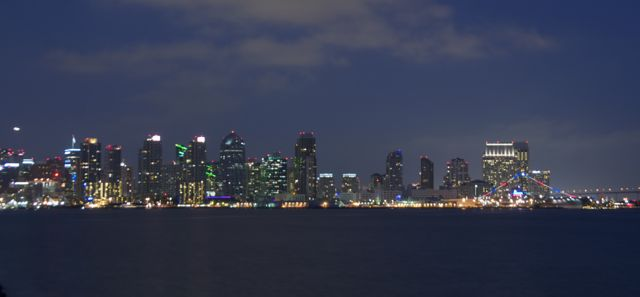
\includegraphics[width=0.5\textwidth]{sandiego}
%  \caption[Short figure caption (must be \protect{$< 4$} lines in the list of figures)]{A picture of San Diego.  Note that figures must be on their own line (no neighboring text) and captions must be single-spaced and appear \protect\textit{below} the figure.  Captions can be as long as you want, but if they are longer than 4 lines in the list of figures, you must provide a short figure caption.\index{SanDiego}} 
%  \label{fig:sandiego}
%\end{figure}
%
%\subsection{A Table Example}
%
%While in Section \ref{ssec:figure_example} Figure \ref{fig:sandiego} we had a majestic figure, here we provide a crazy table example.
%
%
%%%%% TABLE 1 %%%%
%\vspace{0.25in}
%\begin{table}[!ht]
%\caption[Short figure caption (must be \protect{$< 4$} lines in the list of tables)]{A table of when I get hungry.  Note that tables must be on their own line (no neighboring text) and captions must be single-spaced and appear \protect\textit{above} the table.  Captions can be as long as you want, but if they are longer than 4 lines in the list of figures, you must provide a short figure caption.}
%
%\vspace{-0.25in}
%\begin{center}
%\begin{tabular}{|p{1in}|p{2in}|p{2in}|}
%
%\hline
%Time of day & Hunger Level & Preferred Food \\
%
%\hline
%8am & high & IHOP (French Toast) \\
%
%\hline
%noon & medium & Croutons (Tomato Basil Soup \& Granny Smith Chicken Salad) \\
%
%\hline
%5pm & high & Bombay Coast (Saag Paneer) or Hi Thai (Pad See Ew) \\
%
%\hline
%8pm & medium & Yogurt World (froyo!) \\
%
%\hline
%\end{tabular}
%\end{center}
%\label{tab:analysis3}
%\end{table}


\chapter{SPAM: A Secure Package Manager}
\label{ch:spam}

\section{Introduction}
\label{sec:intro}

% Package management systems, as a whole, have to manage an inherent sec issue
Package managers present a security paradox: their job is to make it easy and
secure to pull and install code from the internet.  Uncurated package managers,
package managers that do not impose restrictions on the packages that users
upload, have an even tougher job precisely \emph{because} of this lack of
restriction. Uncurated managers have been wildly successful because
they make it easy to install and publish packages, but they have also been
subject to a number of security flaws. For example, in March of 2014, security
researchers discovered a bug in npm that would allow an attacker complete
control of the registry~\cite{npm-reg-comp}. This attacker, for example, could
replace packages with malicious counterparts or remove packages altogether. A
similar vulnerability in RubyGems came to light when a user uploaded a
proof-of-concept exploit that allowed remote code
execution~\cite{rubygems-reg-comp, github-rubygems}.
% ; RubyGems tried to patch the initial error in 2014 but had to issue another related patch in 2016~\cite{gem-update}.
% @noetzli I am not quite sure that this description is accurate. The initial report is from 2013 and has been patched in 2013.
% The second part mentions a commit from 2014 but i

Most existing uncurated systems focus on reducing risk by securing the
connection between the client and the registry to prevent network attackers
from tampering with registry data in transit; npm and
pip/PyPI~\cite{pypi,npm-https} have both switched to making registry requests
over \texttt{https} over the past few years.
% @noetzli do we need additional cites for RubyGems and pip switching to https?
Similarly, most uncurated package managers check the hash of a package once it has been
downloaded, a request (made over \texttt{https}) meant to ensure the integrity of the downloaded
package~\cite{npm-https}.
% TUF 
These systems do \emph{not} protect against registry compromise,
but recent research addresses this threat. For example, the Diplomat system presents a key-based
method for ensuring the integrity of packages in such an event~\cite{kuppusamy2016diplomat}. 


% These systems are still vulnerable to mal and gov
These systems, though trying to address threats \emph{outside} of the registry
infrastructure, are not secure against internal threats: malicious or negligent
maintainers and developers can compromise the registry ecosystem for all of its users.
For example, in January of 2016, researchers described how evil npm software would
propagate: once downloaded from the registry, this malware would add itself as a dependency
to all of the infected developers' projects~\cite{npm-package-install}.
In a blog post, npm maintainers argue that this is a necessary side-effect of allowing arbitrary install
scripts, and that ``the utility of having installation scripts is greater than the risk of worms.'' 
Furthermore, ``if a large number of users make a concerted effort to publish
malicious packages to npm, malicious packages will be available on npm.'' However, embracing
the dominant attitude of uncurated package managers, they also believe that ``npm is
largely a community of benevolent, helpful people, and so the overwhelming majority of software
in the registry is safe and often useful''~\cite{npm-package-install}.

In contrast, other un- or lightly-curated systems have \emph{not} found their
communities to be full of benevolent, helpful people. The Google Play store
struggles with data-stealing apps~\cite{googleplay-spy}, rooting
apps~\cite{googleplay-root}, and botnet apps~\cite{googleplay-dresscode}.
Infection rates across Android app marketplaces ranged from 0.02\%--0.47\% in
2012, and researchers discovered multiple apps exploiting zero-day
vulnerabilities during the course of this analysis~\cite{zhou2012hey}.  The
Chrome Extension Store faces similar problems: in 2014, Kapravelos et al.
detected 130 malicious and 4,712 suspicious
extensions~\cite{kapravelos2014hulk}.  Malware and adware creators have also
purchased popular Chrome extensions and then pushed automatic, malicious
updates to extension users~\cite{chrome-sale}. 

% pull leftpad for space?
Similarly, registry administrators may not always act---or may be compelled \emph{not} to
act---in the best interests of their users. For example, npm administrators
have re-uploaded packages after they are pulled by developers~\cite{leftpad}.
Many registries are also backed by for-profit
companies\footnote{e.g. npm (npm, Inc.) and Yarn (Facebook)}; trusting these registries
to protect their users is like trusting Pinto-era Ford to protect its drivers---a
gamble at best. Furthermore, even if npm is staffed by
the opposite of Ford execs, governments may compel them to tamper with the registry anyway.
At the request of the US government, for example, Yahoo! included custom backdoors to allow
agencies to search user emails~\cite{yahoo-backdoor}. This surveillance shows
no signs of slowing (e.g., see~\cite{trumptweet}). 

% Our solution
In this chapter, we describe the current state of uncurated package managers,
using npm as a running example. 
Then, we present designs for a community repository and package manager, \spam{},
that limit the ramifications of malicious and negligent users and
administrators. 


\section{Current package managers}
\label{sec:problem}
This section presents an overview of uncurated package management systems and
outlines several security challenges within these systems.  We use the \node
package manager npm as a running example because of its popularity.
The security issues we
describe are neither unique to npm nor specific to \node; most uncurated
language package managers have similar drawbacks.  To illustrate these common
drawbacks, we first describe the workflow of a typical \node developer.

Developer Dan wants to reformat the columns of a CSV file. To get hip with the
times, he decides to use \js and \node, and begins by writing a helper
function that inserts spaces on the left-hand side of a line. The
function is elegant and useful; to share it with others, he adds testing and
benchmarking (pulling in dependencies like the \texttt{tape} library) and
creates a new package named \lpad. 

Dan decides to make the world a better place by publishing \lpad on the npm
registry.  Any developer can install Dan's \lpad package or depend on it within their
own project. Some users may even download \lpad without knowing it; as they
install more popular packages that list \lpad as a dependency, they also
install \lpad itself. Users may even end up with multiple versions of \lpad or
multiple copies of the same version (due to how npm resolves
dependencies)~\cite{npm3deps,npm2deps}. Eventually, fans of \lpad start
bombarding Dan with requests to update and extend his package, so he uploads it
to \gh and syncs his repository with the Travis continuous integration (CI)
cloud service.  Now, tests will run anytime someone creates a pull request or
Dan pushes directly to the repository---\lpad will only contain fast,
functionally-correct code!

Using uncurated package managers, developers are able to build
relatively complex software largely by repurposing existing projects (like Dan's \lpad);
the package manager and registry do not impose restrictions on uploaded code. This
lax security, however, comes at a cost.

\subsection{Malicious registry}
In most uncurated package management systems, all users that depend on a
malicious registry are at its mercy. For example, a registry may
serve malicious or vulnerable packages in place of 
packages the users request. A registry may behave maliciously
even if its administrators are virtuous: admins may be
compelled by the government, network attackers may tamper with
packages via MITM attacks, etc. In fact, in writing this paper, we discovered a
vulnerability in npm that allows a network attacker to intercept
certain installs~\cite{shrink}; developers may explicitly link to their dependencies with
\http instead of \https URLs, putting those who
download their packages at risk. npm maintainers have
not fixed this vulnerability. Instead, they warn developers to manually
stick an ``\texttt{s}'' at the end of those links~\cite{shrink-response}.

\subsection{Malicious developer} % npm v 2: different?
In addition to trusting the registry, developers must also trust the packages
that they install, and those on which their installations depend on. This is
deceptively difficult: even when developers rely on a handful of packages,
their transitive dependency list is an order of magnitude larger---and that
much more difficult to audit. 
We looked at the top 20 npm packages as of January 24, 2015, and found that
the average npm package lists 50 dependencies, with a median of one, a minimum
of zero, and a maximum of 626. 
In practice, this number is sometimes worse; for example, a popular dependency
that many bootcamps include in their skeletons is
\texttt{hackathon-starter}~\cite{hackathon-starter}.
This project downloads 558 dependencies before bootcampers even write a line of app
code.
While NPM suggests installing only trusted packages, this also does not scale
when popular packages like \texttt{lodash} release every thirteen
days, on average~\cite{npm-package-install, staicu2016understanding}.
Furthermore, packages with many dependencies may also include vulnerable
and out of date dependency versions. We analyzed\footnote{
  The measurements and analyses described here are based on a clone of
  the npm registry; we fetched packages between December 6--15, 2016 using
  \texttt{registry-static}~\cite{registry-static}.} all packages by the top ten
authors on npm---presumably trustworthy people---and out of 6,498 projects,
we found that 1,693, or 26.1\% have out of date dependencies.

\subsection{Malicious integration services}
Along with registries and third-party code, developers also place implicit trust in
integration tools like Travis~\cite{travis}. This implicit trust is once again
transitive: for example, when Dan shares his API keys with Travis, he---and
anyone whose package depends on him---is trusting Travis not to publish any
malicious package versions. Furthermore, Dan must properly encrypt his keys
when he shares them with Travis, since continuous integrators are allowed to
use plaintext API keys. Many developers accidentally publish their
API keys publicly: we searched the first 1,000 \gh results for ``provider: npm api\_key.''
and found that 174 of 527 unique \gh developers uploaded a YAML file
with unencrypted API keys. 


\section{Registry design}\label{design}
In this section, we describe our secure package manager (\spam), which intends to
prevent and contain damage even in the presence of malicious users, registry
administrators, and third-party tools like Travis. \spam consists of
a distributed multi-node registry which manages package data and metadata and
provides an interface to update and query this data. \spam also includes a
client tool that allows developers to communicate with the registry.

\subsection{The registry}
At a high level, the goal of the registry is to maintain a ledger
with information about users and packages. The ledger provides
the client tools---and thus the developers who use them---with a way of
verifying the authenticity of data and metadata about packages and other users.
The ledger also serves to provide developers with a single
mechanism for storing package metadata. We use a federated Byzantine
agreement system (\fbas) to ensure that the ledger remains uncompromised in the
presence of malicious actors (e.g., registry administrators or government
mandates)~\cite{stellar}.
% Below, we expand on the ledger system and the
% \fbas{} that ensures its integrity, consistency, and availability. 

The ledger consists of different messages that record
user information (e.g., name registrations and proofs of identity) and
package metadata (e.g., package release information). 
Each entry $e_n$ in the ledger contains the entry number $n$ (a monotonically
increasing number), a new client message $m$, and a hash of the entry number, message and previous ledger entry---i.e., $H(n\|m\|e_{n-1})$.
Therefore, each entry in the ledger securely refers to the previous state of the
ledger.  The message $m$ describes an action (e.g., update package) that the client
has requested of the registry and contains that client's signature. 

For example, to create a new account, a developer executes the \spamuser{} command.
The \spam{} client creates a new user public key pair and sends the
\registeruser{} message to the registry; this message contains the user's public key
and proposed name, signed by their corresponding private key.
If that name is not already taken---if it has not already been recorded in the
ledger---the registry will add the \registeruser request to the ledger.
This record acknowledges that the new name is now associated with the user's key.

There are \numMessages different messages that the \spam client can send to the registry
after interacting with users on the command line that lead to ledger modifications.
\Cref{fig:messages} lists these
messages, most of which are self explanatory, with the exception of the
\proveidentity{} and \extensible{} messages---the latter of which we describe
later on. The \proveidentity{} message allows a user to associate their private key
with their public social networks, therefore tying their \spam identity to an external
identity. For example, a developer will associate his \spam{} key with his
Twitter \texttt{@handle} by publishing a signed Tweet. This allows other
users to verify the authenticity of the developer's packages; furthermore, it
allows other users to install his packages \emph{only if} they trust
him and he has not revoked his key. 

\begin{table*}[ht!]
  \caption[The different messages supported by our registry]{
    The different messages supported by our registry.
    % Every client message $m$ is signed $\langle m\rangle_k$ with key $k$.
    We omit the messages that clients use to retrieve data from the ledger.
  }
\label{fig:messages}
\centering
\small
\begin{tabularx}{\textwidth}{lX}
\toprule
\textbf{Client message}   & \textbf{Description} \\
\midrule
$\langle\registeruser: U, U_{pk} \rangle_{U_{sk}}$ &
  Register a new user $U$ and public key $U_{pk}$ signed with the user's private key $U_{sk}$.\\
%%
$\langle\proveidentity: p, U_{pk}\rangle_{U_{sk}}$  &
  Associate an external identity with user key $U_{pk}$; the proof of identity
  $p$ contains URL(s) to signed social network post(s).  When a registry node
  records this message in its ledger, it asserts to have verified the
  signed post(s).\\
%%
$\langle\langle\registerpackage: P, P_{pk}\rangle_{P_{sk}}\rangle_{U_{sk}}$        &
  Register a new package name $P$ and project keys $(P_{pk}, P_{sk})$.\\
%%
$\langle\langle\replaceprojkey: P, P_{pk}\rangle_{P_{sk}}\rangle_{U_{sk}}$        &
  Revoke existing project key and associate the
  new key pairs $(P_{pk}, P_{sk})$ with project $P$.\\
%%
$\langle\replaceuserkey: U, U_{pk}, p\rangle_{U_{sk}}$ &
  Replace user $U$'s existing key with with key-pair $(U_{pk}, U_{sk})$.
  Here, $p$ contains proofs of identity (as above) for a majority of the $U$'s
  external identities.\\
%%
\midrule
%%
  $\langle\langle\registerprojectkey: P, P_{pk}'\rangle_{P_{sk}'}\rangle_{P_{sk}}$ &
  Add a new collaborator/device key to $P$ by registering their project key $P_{pk}'$.
  $P_{sk}$ must correspond to the project key of the owner or another
  collaborator/device.\\
%%
$\langle\revokeprojkey: P, P_{pk}'\rangle_{P_{sk}}$ &
  Revoke a collaborator/device key $P_{pk}'$.
  $P_{sk}$ must correspond to the project key of the owner or another collaborator.
  If $P_{pk}'$ is the owner's project key, $P_{sk}$ must be the
  corresponding secret key.\\
%%
$\langle\releasepackage: P, v, pkg\rangle_{P_{sk}}$&
  Release a new package version $v$ for project $P$. The package data $pkg$
  contains the actual package tarball (and other metadata). The registry nodes
  record a similar message; instead of the tarball, however, they record the
  URL(s) where the tarball can be downloaded from.\\
%%
$\langle\flagpackage: P, v, f\rangle_{P_{sk}}$&
  Flag version $v$ of package $P$ as $f$ (suspicious or approved), if 
  not already flagged.\\
%%
\midrule
%%
$\langle\extensible: data\rangle_{X_{sk}}$  &
  Add application-specific $data$ to the ledger signed by either project
  or user key $X_{sk}$.\\
\bottomrule
\end{tabularx}
\end{table*}
% maybe group together the upcall dudes like toString.

\subsection{User and package keys}
\spam{} manages all keys automatically to prevent key overuse and
compromise. For example, \spam{} creates a new user key
when a developer creates a new account. \spam{} also
generates a new key each time the user creates a new project, and \emph{only}
that key may sign project updates---the user key cannot sign them.
Users can run other \spam{} commands that create additional keys
associated with a project, allowing them to release projects from multiple
machines or integrate with CI tools like Travis. Compromise of a project key is not equivalent to
compromise of a user's account; a malicious, key-stealing Travis can
only push updates to a single project. Moreover, users can revoke
project keys if they have been compromised.

To revoke a project key, the user runs the \revokeprojkeycmd{} command, which
sends a message, signed with the user key, to the registry. This message
indicates which project key should be revoked. At this point, the user
must approve or flag any past changes to the compromised project
(such as collaborator additions). In practice, this amounts to choosing an
entry number to demarcate the point of compromise. The \spam{} client
displays a list of project changes and asks the user to flag the first
suspicious change, if any. All subsequent changes are
automatically flagged as suspicious. Finally, the \spam client sends
these flag messages to the registry.

To revoke and replace a user key, the user runs the \replaceuserkeycmd{} command, which
consists of several steps. First, the cli tool prompts the user to update
the majority of their external identity proofs with a new key (which is equivalent to
sending a number of \proveidentity messages, atomically). The cli tool
will then notify the registry that the old key is invalid and that the new key is associated
with the same user. By updating the ledger with the \replaceuserkey{} message, the
registry asserts that it has verified the new key with the user's external identities
(e.g., Twitter). Then, the \spam client asks the user to demarcate
a point of compromise, following similar steps to those in the project-key
compromise. 

\subsection{Distributed registry}
Our registry consists of several (at least four) top-level mirrors, or nodes
that use a consensus protocol---specifically, the Stellar Consensus
Protocol (SCP)---to agree on ledger entries~\cite{stellar}.
Like traditional, centralized Byzantine fault tolerant
agreement (e.g., PBFTA~\cite{pbfts}), SCP can guarantee safety and liveness by
relying on a quorum of nodes to come to an agreement; for example, in an
arrangement with four top-level nodes, our system tolerates one failure.
Users can configure the \spam{} cli tool to talk to any one of the top-level
nodes, and users can trust its results as long as they configure it
to receive at least two signed replies from distinct nodes.

SCP, in contrast to PBFTA, allows nodes to choose which other nodes to listen to. 
In combination with other design choices, this allows a node to detect and
attribute attacks in which multiple registry mirrors are colluding.
This is because SCP does not require a majority of nodes to compose a quorum;
instead, nodes choose one of more \emph{quorum slices}~\cite{stellar}.
Every node $n$'s quorum slices must be non-empty and contain $n$ itself.
For $n$ to agree on ledger entry $e$, every node (including $n$) in \emph{one} of
$n$'s quorum slices must communicate that they believe $e$ to be
true. Now, in order for $e$ to be appended to the
ledger, every other node must be convinced by one of its own quorum slices.
Reaching consensus is a multi-phase process, the details of which we omit;
we refer the reader to the SCP paper and Stellar core for details~\cite{stellar,core}.

In our design, the top-level mirror nodes may employ other
second-level nodes as members of other slices. Top-level mirror nodes maintain both
the ledger and a mirror of the registry contents; they track package data and metadata. 
Second-level nodes, in contrast, do \emph{not} store package data.
Rather, they simply maintain a copy of the ledger. Second-level nodes can arbitrarily
join the network (by considering at least two top level nodes to be in their
quorum slice) to add additional oversight.

This additional oversight is not provided by second-level nodes referring
only to the ledger. Rather, all nodes also keep track of a ``rollback safety''
data structure that contains the previous round of signed (SCP-level) messages from nodes in its quorum
slices. Since these messages contain a hash of the ledger entry histories, a signed
message from a node indicates that this node agrees to the entire history of the
ledger. If top-level nodes collude to rollback the ledger history, second-level nodes
will be able to detect this; they will be able to prove collusion by producing
two signed, contradicting messages from a culprit node. One of these messages
comes from the rollback safety buffer and one is the most recent message with
a backdated entry number. 

\subsection{The registry threat model}
In the absence of second-level nodes, our system can only provide strong
guarantees if the majority of top-level nodes are well-behaved. Under
this assumption, we get availability directly from SCP's liveness
guarantees~\cite{stellar}. SCP also ensures the safety of the ledger,
which itself contains signed messages; together, this ensures the integrity
and authenticity of packages.
Every time a developer downloads a package, the \spam{} cli tool verifies that
package's signature. Moreover, the \spam{} cli tool verifies that that package
has not been flagged (e.g., due to key compromise). 

During the time when key is compromised but not yet revoked, our system
cannot protect the developers that download malicious packages signed under
the compromised key. However, \spam's separation of project and user keys and
tie in with external services---e.g., using Twitter for identity
verification---make it possible to recover from key compromises without having
to create a new identify. Even if an attacker steals a user key, they cannot
prevent the user from revoking the key unless they compromise a majority of
that user's external identities (GitHub, Twitter, StackOverflow, etc.). 

In general, our system cannot provide guarantees against users running malicious
code. However, we can attribute malicious packages back to their authors---and,
to a certain extent, to those authors' identities. Furthermore, users can
configure the \spam{} cli tool to only install packages authored by developers
that the user explicitly trusts---a restriction that may be imposed on sub-dependencies
as well. Though this simple white-list policy is easy to ship in an early release of
\spam, we envision eventually extending the cli tool with more interesting policies.
For example, we can take advantage of the fact that \spam users are already
connected to social graphs (e.g., Twitter) to compute a level of trustworthiness.
Even if Eve creates fake Twitter and GitHub identities, she will have to
cultivate real friendships in order to appear legitimate~\footnote{Here again
  we can leverage the idea of quorum intersection from SCP to
  ensure that even if Eve creates thousands of followers, if none intersect
  with other peoples' graphs, she will still appear suspicious.}.

Without second-level nodes, a quorum of top-level mirror nodes can collude to carry out
a number of attacks. For example, they can revoke and replace a user's key by appending
a \replaceuserkey message to the ledger, signing it with a new, fake user-key.
This is possible even without compromising the user's Twitter or GitHub accounts,
because the onus of verifying identity is on the registry itself. Colluding
nodes can also roll back ledger history to, for example, conceal backdoors.

With second-level nodes, on the other hand, our system is able to detect
rollback attacks and attribute them to malicious nodes. As long as a first- or
second-level node is not colluding, this node can prove that other nodes have
colluded. Using the rollback safety mechanism, the honest node identifies any
contradictions in any lying node's version of history. Even if all nodes except
for one are colluding, honest, second-tier nodes will still see externalized
messages which can be used to prove that the colluding first-level nodes in
their quorum slices have said contradicting things.
This alone, however, does not prevent key revocation attacks.

We can extended our system via the \extensible message to both detect key
revocation attacks and attacks wherein colluding nodes upload backdoored
packages only to remove them from their registries shortly after.
If third-party services (e.g., the Internet Archive, ACLU, or EFF) are willing to commit to hosting signed
packages and copies of signed social network messages, they can use the \extensible message
to state their purpose in the ledger. The ACLU, for example, might say that it is willing
to host this data for a certain period of time. Then, every time a package is
released or an identity is proven, the ACLU will store the package
or verification data on its servers and use the \extensible message to state that it has done
so. Such services enable second-level nodes to verify 
that the ledger's claims about key revocations and the contents of packages are
replicated on the ACLU service. If registry nodes collude to
revoke someone's key, the ACLU will not be able to replicate any
social network data, since this data does not exist. If the \spam{} cli tool does
not see a such an identity proof nor a (verifiable) confirmation of
revocation from ACLU, it can be configured to treat the new key
as compromised: it will refuse to trust anything that the key has signed.
A similar process can be used to ensure that registry nodes are not colluding to
conceal backdoored packages. 

\subsection{Limitations}
Our system design, naturally, comes with limitations.
%
For example, our design does not prevent front-running attacks. These attacks
occur when, for example, a developer tries to register a user name but
is communicating with a malicious registry node. The malicious node
will receive the user request but instead request the user's chosen name
on behalf of an attacker. 
Once the attacker has successfully registered the name, the malicious node will
handle the developer's request as usual---ensuring its denial.
This problem is not an artifact of our design~\cite{frontrunning}.

Our design also explicitly does not allow users to transfer user or project
names to others (without essentially giving up on their social network identities as well).
%
Though we believe that such extensions are possible, providing such
``features'' in the presence of nation-state adversaries and key
continuity---i.e., the ability to easily replace compromised keys---remains an
open problem.


\section{Related work}
\label{sec:related}

% This is probably too long and needs some comparison with our design
% Note:
% - They only deal with package integrity and not much else
% - Initial set of root keys have to be trusted
% - There is no real solution for managing dev/project relationships
%
Cappos et al.~\cite{cappos:look} identified the dangers of compromised
or malicious package managers and registries.
%
The Update Framework (TUF)~\cite{samuel2010survivable} and the
Diplomat~\cite{kuppusamy2016diplomat} package managers---related work closest to
ours---follow up on~\cite{cappos:look}, borrowing ideas from Tor's update
framework Thandy~\cite{thandy}.
%
TUF guarantees package integrity by (1) using multiple keys
to sign any package data and (2) assigning roles to keys so that one key cannot
be used to sign off on different kind of data (e.g., one project's key cannot
be used to sign another's releases).
%
Diplomat further extends TUF with a key hierarchy, maintained by the registry,
to address an important concern---how to retrofit existing package manager design with
security.
%
We adopt the idea that user keys and project keys should be separated from
these frameworks.
%
Unlike these systems, however, we do not assume registry administrators to be
trusted---our attacker model is considerably stronger.
%
This naturally comes at the cost of not being easy to retrofit on top of
existing, insecure systems.

Keybase~\cite{keybase} pioneered the idea of tying public keys with online
identities.
%
Our system uses this same idea to provide key continuity.
%
Though we do not rely the PGP web of trust that Keybase builds on---our design
is considerably simpler~\cite{openbsd}---we believe that a similar idea of
following or endorsing users on \spam can potentially prove useful in assigning
a level of (dis)trust to downloaded packages.
%
For example, if a developer installs a package that is signed by a user that is
not followed by anybody that the developer follows/endorses, the \spam cli can
warn before continuing with the install---potentially preventing typosquatting
attacks.

% signing packages with a subset of multiple keys in various roles that can be
% delegated.  We draw from TUF by providing keys per package that are then linked
% to a user, but unlike TUF we do not require multiple signatures to verify a
%
% There has been other work on secure package manager design --- we review some of
% these designs here in brief detail and how they relate to our system.  For
% example, the Update Framework (TUF)~\cite{samuel2010survivable} is a framework
% whose main purpose is to guarantee the integrity of packages. This is done by
% signing packages with a subset of multiple keys in various roles that can be
% delegated.  We draw from TUF by providing keys per package that are then linked
% to a user, but unlike TUF we do not require multiple signatures to verify a
% package.  Diplomat~\cite{kuppusamy2016diplomat} which builds off of TUF, adds
% security models to provide a sense of usability and flexibility to the package
% manager. It is important to note that the repo admins in the Diplomat scheme
% need to provide regular maintenance in order to ensure that new packages are
% verified and also to revoke project keys if they are compromised --- this adds
% unnecessary work on the repo admins. In our system, we automate this work with
% our cli tool. Moreover, our system uses links to various third-party services to
% verify a users identity with their keys. This is a similar design to
% Keybase~\cite{keybase}, which is a system that links users public keys to their
% identities by directly linking their key to various social-media platforms.

% \todo{Byzantine}
% \todo{SCP}
% \todo{nixOS}
% \todo{privacy mirror}

%TUF
%The main purpose of the framework is to
%guarantee the integrity of packages, which is done by signing packages with one
%or multiple keys. To minimize the impact of a compromised key, there are
%multiple roles with different responsibilities (e.g. roles for signing packages
%and a role for publishing the timestamp of the most recent change). Each role
%has their own key and trust in keys is established by delegation from a root
%role. The security of the system depends on the keys for the root being
%uncompromised.
%
%Diplomat TUF - how they still
%leave stuff to admins, no help for
%comrpomise in a transparent way
%
%can do this with blockchain


\section{Acknowledgements}
\label{sec:acknowledgement-spam}
\Cref{ch:spam}, in part is currently being prepared for submission for
publication of the material. Brown, Fraser; Mirian, Ariana; Jaiswal, Atyansh;
N\"otzli, Andres; Stefan, Deian. The dissertation/thesis author was a
co-author of this material.



%% APPENDIX
\appendix
\chapter{Final notes}
What to do about things.  What did he say.
  Remove me in case of abdominal pain.



%% END MATTER
% \printindex %% Uncomment to display the index
% \nocite{}  %% Put any references that you want to include in the bib 
%               but haven't cited in the braces.
\bibliographystyle{alpha}  %% This is just my personal favorite style. 
%                              There are many others.
%\setlength{\bibleftmargin}{0.25in}  % indent each item
%\setlength{\bibindent}{-\bibleftmargin}  % unindent the first line
%\def\baselinestretch{1.0}  % force single spacing
%\setlength{\bibitemsep}{0.16in}  % add extra space between items
\bibliography{thesis}  %% This looks for the bibliography in template.bib 
%                          which should be formatted as a bibtex file.
%                          and needs to be separately compiled into a bbl file.
\end{document}

